In questo esperimento si vuole implementare la funzione soft-start di un LED. Essa impone al LED di accendersi e spegnersi in un determinato intervallo di tempo, modificando la sua potenza luminosa gradualmente. Il programma funziona in questo modo: quando viene premuto il tasto una volta, la potenza ottica del LED cresce gradualmente da 0 al valore massimo (in 2 secondi). Quando il tasto viene premuto nuovamente, la potenza ottica del LED decresce gradualmente da 0 al valore minimo (in 2 secondi). Il funzionamento è rappresentato in Figura \ref{fig:Graph1}.
\begin{figure}[H]
    \centering
    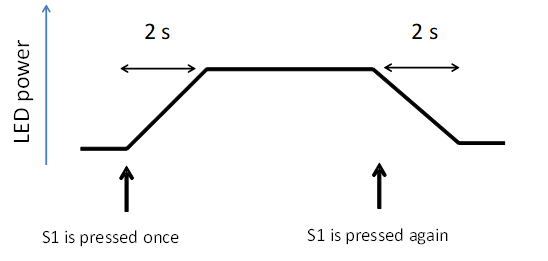
\includegraphics[width=0.6\linewidth]{images/Graph1.png}
    \caption{Funzione soft-start del LED}
    \label{fig:Graph1}
\end{figure}
Per questo esperimento sono stati utilizzati  i seguenti componenti:
\begin{itemize}
    \item Resistenze $R_1=470\text{ }\Omega,R_2=10\text{ k}\Omega, 0.25\text{ W}$
    \item LED 5mm, codice \textit{C503BRANCA0B0AA1}, Cree
    \item Scheda Arduino DUE
    \item Interruttore
\end{itemize}
Il circuito riportato in Figura \ref{fig:Circuit1} è alimentato mediante porta USB del PC, la quale eroga circa $(\sim 5 V)$
\begin{figure}[H]
    \centering
    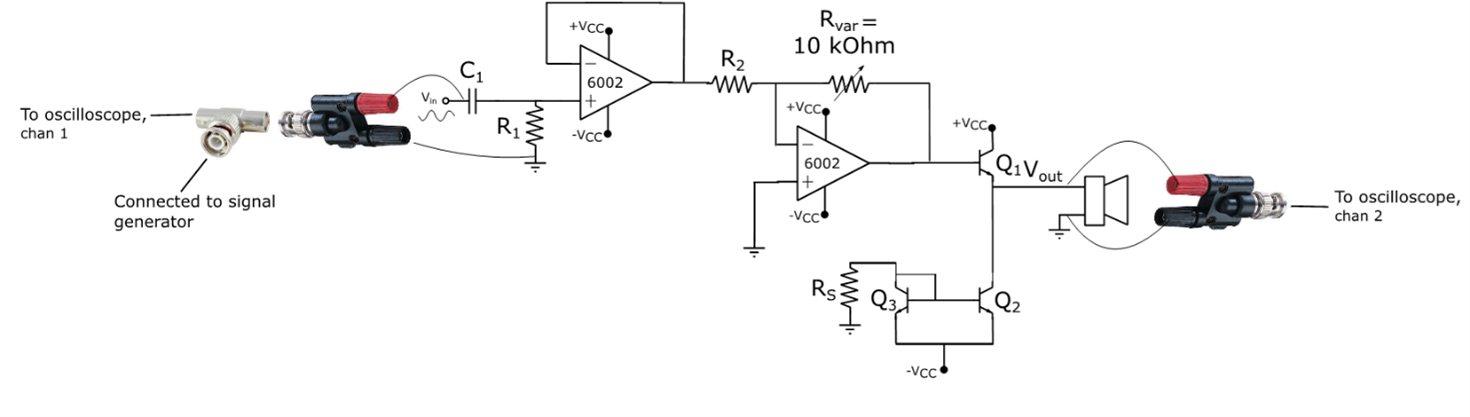
\includegraphics[width=0.4\linewidth]{images/Circuit1.png}
    \caption{Schema circuito}
    \label{fig:Circuit1}
\end{figure}
Il pulsante è collegato al pin digitale \textbf{2} mentre il LED è collegato al pin digitale \textbf{12}.
\subsection{Dimensionamento circuito e analisi - prelab}
La tensione operativa del LED, ricavata dal datasheet vale 
\begin{equation*}
    V_{ON.LED}=2.1\text{ V}
\end{equation*}
La massima corrente erogabile dal pin 12 di Arduino DUE è 
\begin{equation*}
    I_{OUT.MAX}=3\text{ mA}
\end{equation*}
Il valore della resistenza $R_1$ è stato determinato in base ai dati reperiti dalle specifiche dei componenti, essa ha lo scopo di \underline{limitare la corrente uscente dalla scheda}.
\begin{equation}
    R_1=470\text{ }\Omega\implies I_{OUT}=\frac{3.3V-V_{ON.LED}}{R_1}\approx2.5\text{ mA}
\end{equation}
La resistenza $R_2$, detta di \textit{pull-down} è utilizzata per evitare che la lettura del pin digitale rimanga a valori flottanti, il valore $R_2 =  10\text{ k}\Omega$ permette di ridurre al minimo la corrente erogata dal pin di alimentazione e allo stesso tempo un rapido assestamento della tensione.
\subsection{Codice}
Il pin digitale \textbf{12} è un pin di tipo "PWM" per tanto è possibile con esso controllare direttamente la potenza sul LED. Infatti la potenza (media) sarà direttamente proporzionale al segnale PWM.\\
Il codice è stato realizzato costruendo due funzioni \texttt{fade\_in()} e \texttt{fade\_out()} che implementano lo "slow-start" del LED come in Figura \ref{fig:Graph1}. E' stato inserito un tempo di debounce di $5\text{ ms}$ tramite \texttt{delay(5);} per garantire una corretta lettura del segnale proveniente dal pulsante. Vengono inoltre utilizzate variabili costanti per i numeri dei pin dei led e alcune variabili booleane per memorizzare lo stato dei led. 
\begin{lstlisting}[frame=single, language=Arduino]
const int buttonPin = 2; // the number of the pushbutton pin
const int ledPin =  12;  // the number of the LED pin
bool buttonState = HIGH; // reading the pushbutton status
bool lastButtonState = HIGH;    // storing the last button state
int timeToFade = 2000;   // time in milliseconds to fade brightness

void setup() {
    pinMode(ledPin, OUTPUT);    //init. LED pin as an output
    pinMode(buttonPin, INPUT);  // init. the button pin as an input
    analogWrite(ledPin,0);  // initialize the LED state as low
}

void loop(){
    buttonState = digitalRead(buttonPin);   // read the button state
    delay(5);   // Debounce time
    if(buttonState){    // Check if the pushbutton is pressed.
        if (lastButtonState == LOW){
            fade_in();  // turn LED on:
            lastButtonState = HIGH;
        } else {
            fade_out(); // turn LED off
            lastButtonState = LOW;
        }
    }
}

void fade_in(){ // 
    for (int ledBright = 0; ledBright <= 255; ledBright++) {
        analogWrite(ledPin, ledBright);
        delay(timeToFade / 255);
    }
}

void fade_out(){
    for (int ledBright = 255; ledBright >= 0; ledBright--) {
        analogWrite(ledPin, ledBright);
        delay(timeToFade / 255);
    }
}
\end{lstlisting}
La funzione \texttt{delay(timeToFade / 255);} serve a regolare la velocità dell'accensione del LED\\\\
E' possibile apprezzare il funzionamento del circuito dal video al \href{https://mediaspace.unipd.it/media/Esperimento+1/1_9uu86mks}{seguente link}